\subsection{Motivation and Relevance of Anomaly Detection in Electric Vehicle Supply Equipment}

Electric Vehicle Supply Equipment (EVSE) has gained significant importance in recent years \cite{paper_relevance_EVSE}. Analyzing the market sales of electric vehicles (EVs), a remarkable growth can be observed. In 2012, only 120,000 EVs were sold, whereas by 2021, sales had surged to nearly 6.6 million. To achieve net-zero CO2 emissions by 2050, as planned by the European Union \cite{EU2050}, the number of EVs must continue to rise substantially, requiring an 11-fold increase from current levels by 2030 \cite{Number_of_EVSE_sales}.\\
To manage the much higher demand for EVs on public roads, it is expected that the market for EVSE will grow similarly to the sales of EVs \cite{ladeinfrastruktur}. The correlation between the number of EVs and the number of EVSE is high. Market data from the last few years show that the top four countries in the European Union, such as Germany, the Netherlands, France, and Belgium, with the best EVSE infrastructure, are also the top four with the largest market share of EVs \cite{ladeinfrastruktur}.
\begin{figure}[htbp]
  \centering
  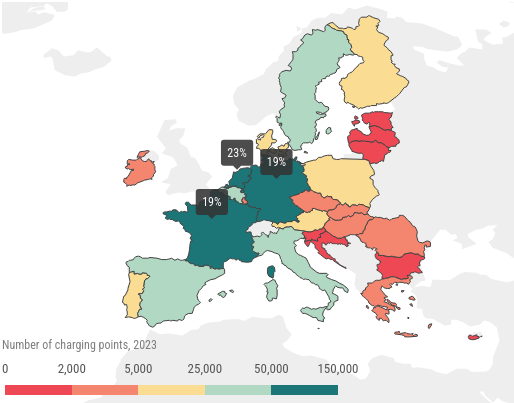
\includegraphics[width=0.5\textwidth]{pics/chargingPointsInfrastructure.png}
  \caption{Availability of public charging points and market share of electric cars in the European Union \cite{ladeinfrastruktur}.}
  \label{fig:chargingPointsInfrastructure}
\end{figure}
\\
With the growing number of EVSE, particularly Charging Stations (CS), the interest of cyber-criminal groups in attacking these systems is also increasing \cite{silicon_evse_attacks}. At first glance, EVSE systems may not appear to be direct targets for accessing critical data or manipulation. Upon closer examination, it turns out that they can serve as entry points to gain access to more sensitive or private information \cite{nature2025}. The following figure illustrates how EVSE components, such as charging stations, can act as access nodes to critical or private data.
\begin{figure}[H]
  \centering
  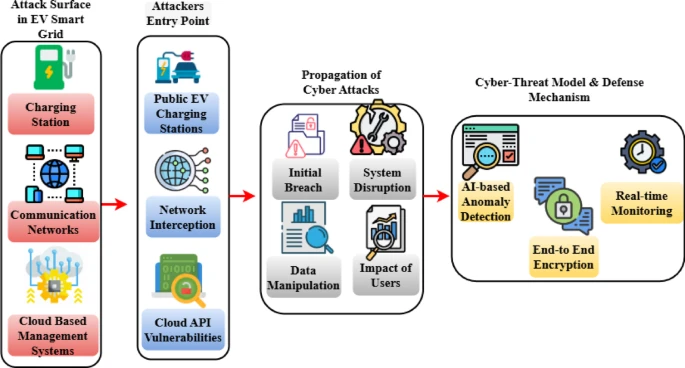
\includegraphics[width=0.7\textwidth]{pics/EVSE_attackpoints.png}
  \caption{Electric Vehicle Supply Equipment as an access node to critical data \cite{nature2025}.}
  \label{fig:EVSE_attackpoints}
\end{figure}

With access to these kinds of data, critical attacks, such as data manipulations, data theft, disruption of service, or even complete system failure, are possible \cite{nature2025}. This does not only lead to a high financial risk, but it also affects the trust of users in EVSE systems and potentially slows down the adoption of EVs in general.\\
If end users are provided with a stable and secure EVSE infrastructure, consumer confidence in switching to electric vehicles will be significantly higher. This ensures, in turn, consistent growth in the adoption of both EVs and EVSE systems \cite{evse-cybersecurity2025}.\\
As outlined in the first paragraphs, the rapid growth of EVs and EVSE infrastructure also requires a robust monitoring and anomaly detection system to safeguard the security of the EVSE infrastructure. Only by guaranteeing a secure EVSE environment can user trust in the energy transition be maintained and major cybersecurity incidents in the future be avoided.\\

Ensuring high security standards for EVSE systems is of critical importance, but difficult to achieve. The EVSE infrastructure constitutes a complex system that includes not only charging stations but also sophisticated backend systems and communication protocols. These components and software solutions are typically developed, published, and maintained by various vendors, which makes securing the entire system a challenging task.\\
Combining all the different software from vendors into a secure infrastructure is challenging enough, but the EVSE infrastructure, especially charging stations (CS), is also regularly installed in public places. Even when not in a public setting, these installations are often outdoors, where security measures are significantly lower than in buildings protected by walls, doors, and other physical barriers.\\
In this paper, the focus is on wallboxes, which are generally smaller than CS and are typically used in private settings. They are often installed directly on house walls or in garages, and thus still form part of the overall EVSE infrastructure.\\
The fact that they are installed in private areas initially suggests a higher level of security. However, since these areas are still outdoors, it must be assumed that there are no additional physical security measures beyond the wallbox itself. It is crucial to develop a system that not only protects against software-based attacks, such as Denial-of-Service (DoS) or Distributed Denial-of-Service (DDoS), but also considers other potential attack vectors, such as firmware manipulation and unauthorized data interception. In addition, the system has to secure the hardware against physical threats, like tampering, theft, or other intrusions.\\

In this project, wallboxes from the \textit{ReSiLENT} \cite{ReSiLENT} project, provided by \textit{Stöhr Mobility GmbH} \cite{StoehrMobility}, are used. The software is developed by \textit{ChargeIQ GmbH} \cite{ChargeIQ} and already includes basic security measures to protect against external threats. This project is also carried out in cooperation with \textit{ASVIN GmbH} \cite{ASVIN}. In the following chapter, the internal components of the wallbox are examined more closely.\\

\begin{figure}[H]
  \centering
  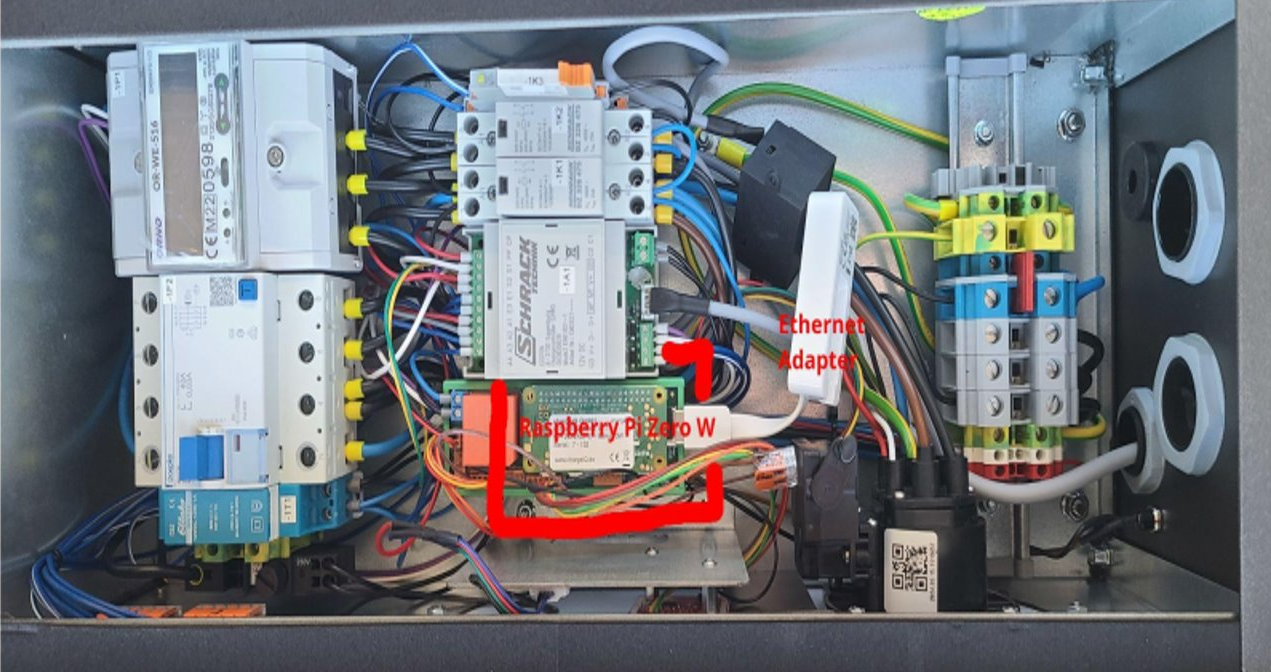
\includegraphics[width=0.7\textwidth]{pics/wallbox.png}
  \caption{Interior view of the wallbox \cite{wallbox}.}
  \label{fig:Wallbox}
\end{figure}

In this figure, the internal components of the wallbox are visible. The wallbox is equipped with a Raspberry Pi Zero W, which is responsible for communication with the backend, including the transmission of user data and handling of payment processes from the charging process. This component is secured and programmed by \textit{ChargeIQ GmbH} \cite{ChargeIQ}.\\
The sensitive hardware components are enclosed in an aluminum casing designed by \textit{Stöhr Mobility GmbH} \cite{StoehrMobility}, which provides a degree of protection against physical attacks.\\
As already mentioned, the wallbox also processes personal data of users, such as their user ID and payment information, in communication with the backend server. This requires special attention in the context of the DSGVO / GDPR, as additional requirements for the protection of personal data, such as data minimization, storage limitation \cite{DSGVOart5}, and legal obligation \cite{DSGVOart6}, must be taken into account throughout the entire EVSE infrastructure.\\

Security requires significant computational resources, particularly in the domain of anomaly detection. As shown in Figure~\ref{fig:Wallbox}, the wallbox is equipped with a Raspberry Pi Zero W, which offers sufficient resources for a single-board computer. However, when processing and analyzing over 900 hardware events to detect potential anomalies, the system quickly reaches the limits of its hardware capabilities. This is just a small example of the challenges faced in securing EVSE infrastructure.\\
Due to the combination of digital and physical threats, the involvement of multiple vendors, and strict data protection requirements, securing Electric Vehicle Supply Equipment (EVSE) infrastructure is a complex task and entails numerous challenges.